\section{Introduction}

The IEC 61850 information model 
is classified as a  
\glsentrytext{O-O} system. Is necessary 
to have a clear understanding of \gls{O-O} technology
to dive into IEC 61850 object modelling. 
For this reason this chapter describes 
the \gls{O-O} technology
on which the IEC 61850 information model 
has been standarized\todo[inline]{No se si esta 
bien escrita la palabra standarized}. 

The chapter does not describe all the \gls{O-O} principles, 
just \todo{traduccion:�just focuses or focuses just?} focuses 
on the neccesary
background to understand the IEC 61850 
information model. 
The sections which follow will define the 
background which the IEC 61850 
object oriented information system 
was constructed, both formally 
and through examples.
A detailed description of the \gls{O-O} fundamentals  
and reference materials are provided. To achieve a 
robust concepts comprehension a practical 
implementation with the%the Unified Modeling Language 
\gls{UML} 
\todo{agregar al glossaries} 
\cite{UML2:2009} 
and Java \cite{Java:specification} are provided. 
This chapter is very
practical in the sense that uses language programmings to model 
very carefully selected models  
used by the IEC 61850 standard, 
(but not explaining explicitly nothing 
about the standard yet!).
This chapter is destined 
for electrical engineers and professionals of 
related areas readers which the \gls{O-O} software construction 
is not part of the curriculum. For this reason, 
the practical examples uses electricity area 
elements. The readers with a strong knowledge 
of programming could skip this
chapter \todo[inline, color=blue!50!red!50]{
	deber\'ia agregar esta ultima frase?:
	\emph{The readers with a strong knowledge 
	of programming could skip this
	chapter}
}




\todo[inline]{En este cap�tulo voy a agregar 
los graficos a continuacion:

(los ejemplos que voy usando son con estas clases)}


\begin{figure}
  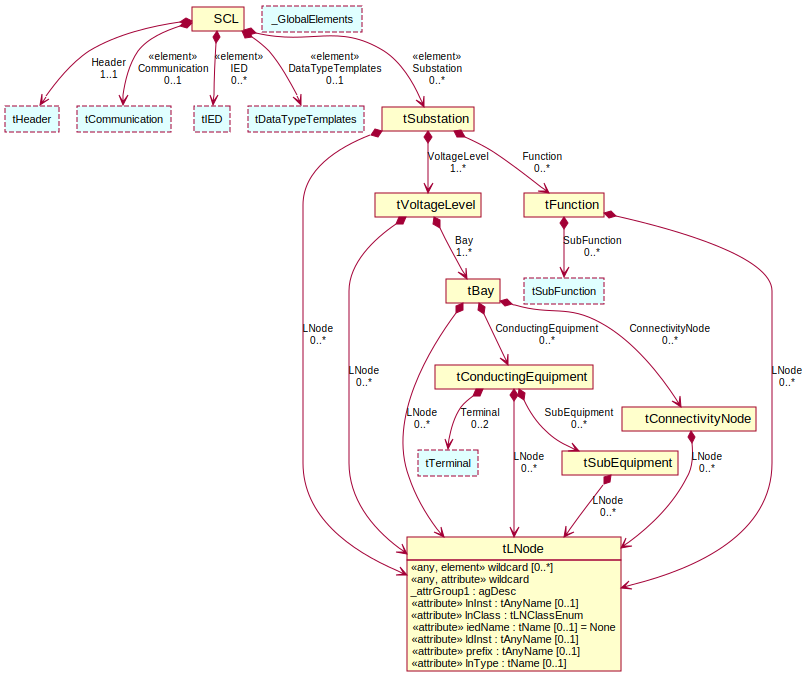
\includegraphics[width=1.0\textwidth]{chapters/ch-oop/figures/LogicalNodeAllocationStructure}
  \caption{Logical Node and their role at the substation level}
  \label{fig:LogicalNodeAllocationStructure}
\end{figure}

\begin{landscape}
	\begin{figure}	
	  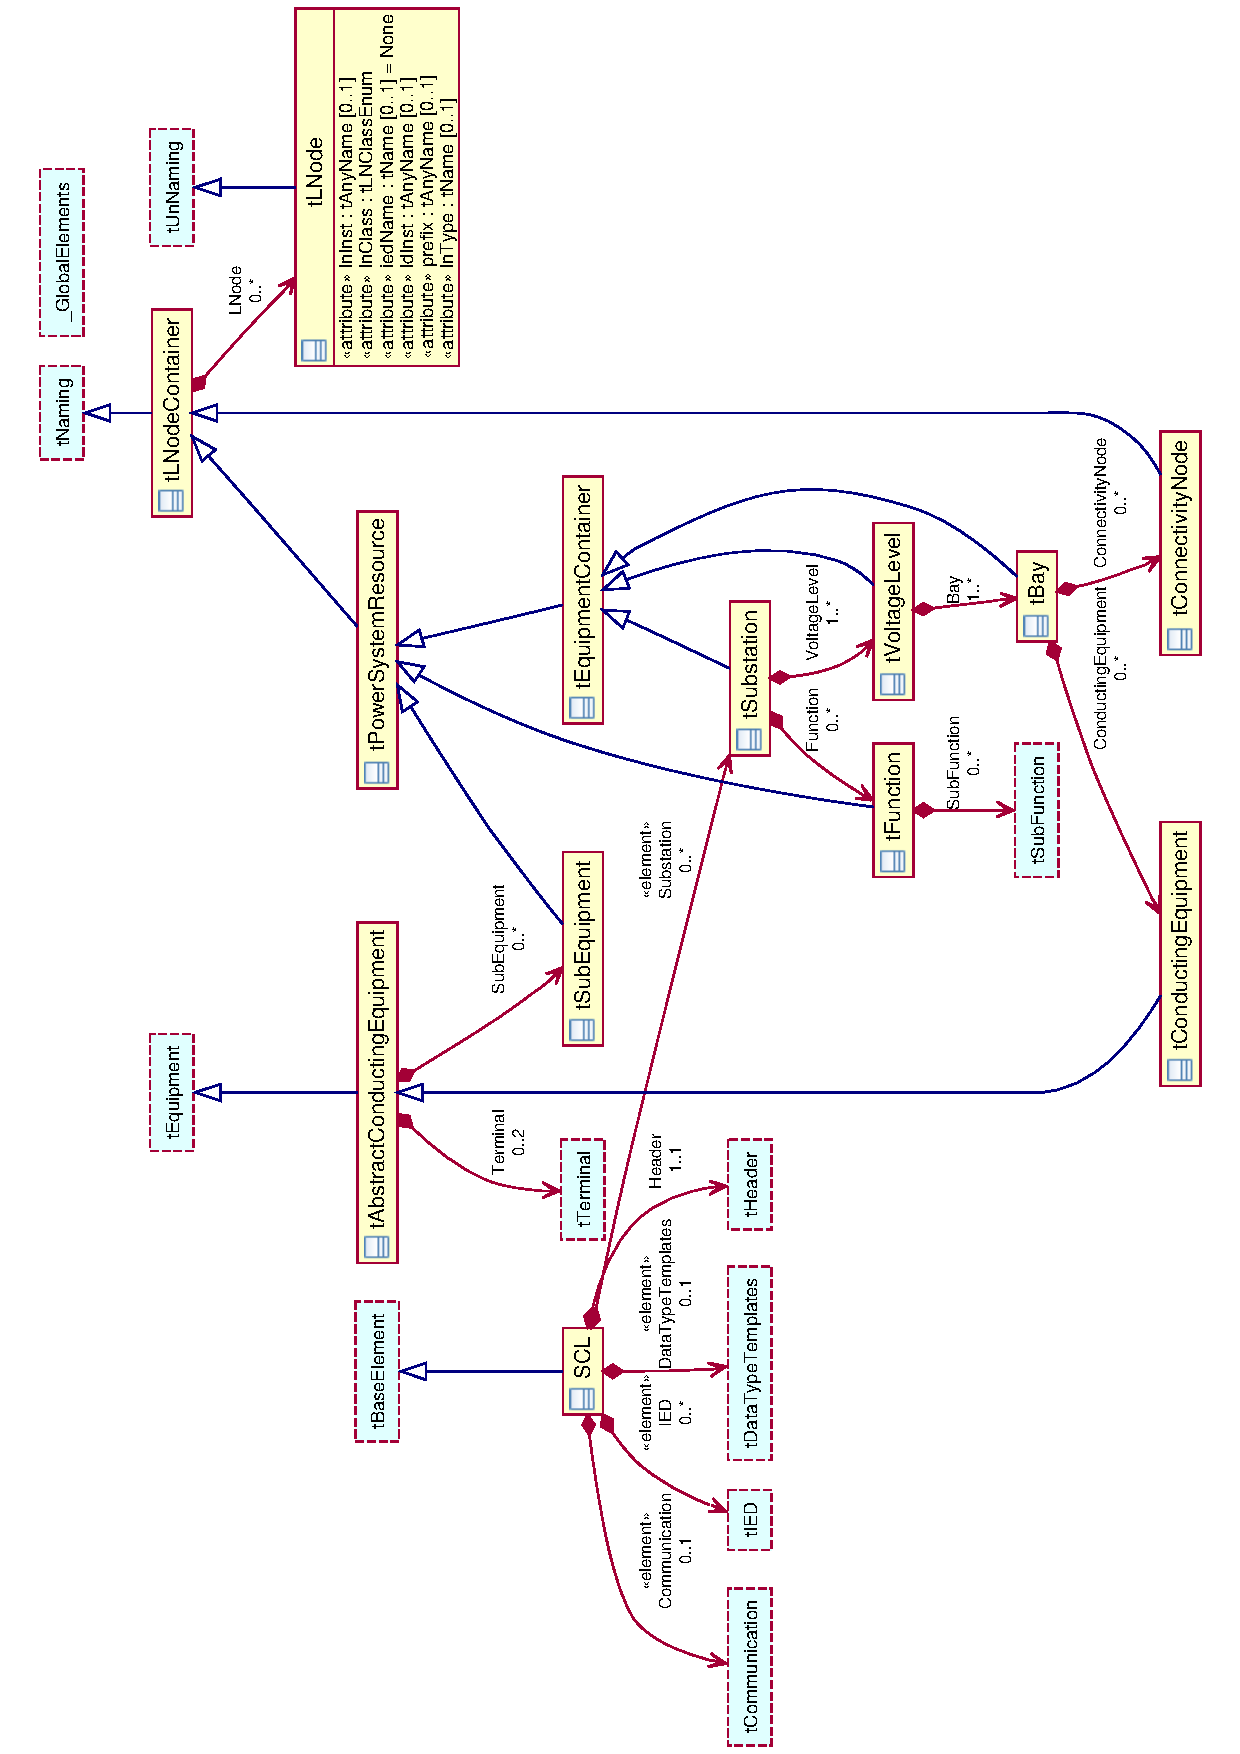
\includegraphics[angle=-90, width=1.0\linewidth]{chapters/ch-oop/figures/LogicalNodeAllocationStructure_with_heritance}
	  \caption{Logical Node and their role at the substation level, depicted with
	  the heritance details}
	  \label{fig:LogicalNodeAllocationStructure_with_heritance}
	\end{figure}
\end{landscape}
	